\documentclass[english, dark, index]{Iart}

\usepackage[]{IMTtikz}

\title{Some short notes on combinatorics}
\subtitle{A handful of notes based on IMPA's combinatorics course, lectured by Robert Morris}
\date{January 16, 2021}

\author{Isabella B}

\newtheorem{theorem}{Theorem}[part]
\newtheorem{corollary}{Corollary}[theorem]
\newtheorem{lemma}{Lemma}[theorem]
\newtheorem{definition}{Definition}[part]
\newtheorem{example}{Example}[chapter]
\newtheorem{conjecture}{Conjecture}[chapter]
\newtheorem{proposition}{Proposition}[chapter]
\let\oldemptyset\emptyset
\let\emptyset\varnothing
\DeclareMathOperator{\ex}{ex}
\DeclareMathOperator{\Var}{Var}
\DeclarePairedDelimiter\ceil{\lceil}{\rceil}
\DeclarePairedDelimiter\floor{\lfloor}{\rfloor}

\begin{document}
	
	\maketitle
	
	\part{Introduction}
	
	\chapter*{Preface}
	
	These notes should deal with some select types of problem, such as
	\begin{enumerate}
		\item Extremal problems
		
		Basically number problems, in which we want boundaries for certain subsets.
		
		\item Counting problems
		
		Which are the classic ``how many'' problems. They are usually extensions of the former type of problem.
		
		\item Probabilistic problems
		
		In which a counting problem has some random component.
	\end{enumerate}

	\chapter{Some motivational problems}
	
	\section{Extremal problems}
	
	Here we introduce two problems which make use of the pigeon-hole principle, which states:
	
	If we have $ I=\set{a_1,a_2,\ldots,a_n} $ items and $ K=\set{b_1,b_2,\ldots,b_m} $ categories, such that $ m<n $ (both natural numbers) then it must be the case that, for some $ b_i $ we have $ a_j,a_k\in b_i $.
	
	So, then, how is it useful for any significant proof?
	
	\begin{example}
		Let $ A\subset \set{1,\ldots,2n} $, then
	\end{example}
	
	% TODO
	\TODO{finish this (problems in lecture \#01)}
	
	\section{Counting problems}
	
	
%	Suppose we have $  $

%	\chapter{}

	\section{Probabilistic problems}

	\chapter{Ramsey Theory}
	
	So, we begin this chapter with the following question:
	
	Suppose we want to arrange a party in which there are either:
	\begin{enumerate}[label=(\alph*)]
		\item \textbf{three} people that \textbf{don't} know each other, or;
		\item \textbf{three} people that \textbf{DO know }each other.
	\end{enumerate}
	And they might seem as very different problems, but if we imagine each relationship as being represented by a coloured line connecting two people (e.g. a blue line if they know each other and a red line if they don't) we can see that colours are arbitrary, and so we could determine their relationship by a coin toss and it wouldn't make a difference.
	
	So, what might this lowest number of people ($ n $) be? Well, if we have $ 5 $ people at a party we could have, say, this:
	
	\begin{center}
		
		\begin{tikzpicture}
			\foreach \x in {1,...,5}
				\coordinate (a\x) at ({(\x+0.25)*360/5}:2);
			
			\draw[cyan] (a1) -- (a3) -- (a5) -- (a2) -- (a4) -- cycle;
			\draw[red] (a1) node[above] {$ p_1 $} -- (a2) node[left] {$ p_2 $} -- (a3) node[below left] {$ p_3 $} -- (a4) node[below right] {$ p_4 $} -- (a5) node[right] {$ p_5 $} -- cycle;
			
			\foreach \x in {1,...,5}
				\fill (a\x) circle (1pt);
			
		\end{tikzpicture}
		
	\end{center}

	In which each person is represented by a dot, and each line represents a relationship.
	
	Then, we can clearly see that no single person knows (or doesn't know) more than 2 others, and we have a counter-example for $ n=5 $.
	
	But then, maybe $ n=6 $, and indeed it is the case!
	
	So how do we prove it? We can make a nice construction for this case:
	
	\begin{theorem}
		$ R(3)=6 $
	\end{theorem}

	\begin{proof}
		Draw $ 6 $ vertices and notice that, by selecting any of them, we colour at least two vertices with the same colour:
		
		\medskip
		
		\begin{multi}
			
			\centering
			\begin{tikzpicture}
				\foreach \x in {1,...,6}
					\coordinate (a\x) at ({(\x+1)*360/6}:2);
				
				\draw[cyan] (a1) -- (a2) (a1) -- (a4) (a1) -- (a6);
				\draw[red] (a1) -- (a3) (a1) -- (a5);
				
				\foreach \x in {1,...,6}
					\fill (a\x) circle (1pt);
			\end{tikzpicture}
			
			\nextcol
			
			\centering
			\begin{tikzpicture}
				\foreach \x in {1,...,6}
				\coordinate (a\x) at ({(\x+1)*360/6}:2);
				
				\draw[cyan] (a1) -- (a2) (a1) -- (a6);
				\draw[red] (a1) -- (a3) (a1) -- (a4) (a1) -- (a5);
				
				\foreach \x in {1,...,6}
				\fill (a\x) circle (1pt);
			\end{tikzpicture}
			
		\end{multi}
	
		Let's select any $ 3 $ edges which are monochromatic say, the middle ones in the rightmost drawing, and then we can see that:
		
		\medskip
		
		\begin{multi}
			
			\centering
			\begin{tikzpicture}
				\foreach \x in {1,...,6}
				\coordinate (a\x) at ({(\x+1)*360/6}:2);
				
				\draw[cyan!30!papercolor] (a1) -- (a2) (a1) -- (a6);
				
				\draw[cyan] (a3) -- (a4) -- (a5) -- cycle;
				\draw[red] (a1) -- (a3) (a1) -- (a4) (a1) -- (a5);
				
				\foreach \x in {1,...,6}
				\fill (a\x) circle (1pt);
			\end{tikzpicture}
		
			\medskip
			
			In case we draw everything in the other colour, we end up forming a triangle.
			
			\nextcol
			
			\centering
			\begin{tikzpicture}
				\foreach \x in {1,...,6}
				\coordinate (a\x) at ({(\x+1)*360/6}:2);
				
				\draw[cyan!30!papercolor] (a1) -- (a2) (a1) -- (a6);
				
				\draw[cyan] (a3) -- (a4) -- (a5);
				\draw[red] (a1) -- (a3) (a1) -- (a4) (a1) -- (a5) (a3) -- (a5);
				
				\foreach \x in {1,...,6}
				\fill (a\x) circle (1pt);
			\end{tikzpicture}
		
			\medskip
			
			If we try to avoid that by changing any one of the edges we form a triangle anyway.
			
		\end{multi}
	\end{proof}

%	\bigskip

	\section{Some straightforward results}

	So, now we can prove a little theorem which is going to be useful to prove another:
	\begin{theorem}[Ramsey's theorem]\label{thm:ramsey}
		If $ c:\binom{\mathbb{N}}{2}\longrightarrow \set{1,\ldots,r} $ then there exists $ A\subset\mathbb{N} $, such that $ A $ is infinite and $ c(\set{a,b})=k\quad\forall a,b\in A,a\neq b $, in which $ k\in\set{1,\ldots,r} $ is constant.
	\end{theorem}

	%TODO
	\TODO{review notation and terminology}

	Before we prove this, let's define some terminology:
	A function that takes some set (in this case the set of all pairs of integers) into some \textit{other(?)} finite set (i.e. attributes a specific value to each member of a set) is called a \term{colouring}.
	
	Let's denote the colour of a pair by $ c(\set{a,b}) $. In this problem we want to find an infinite set of pairs which are \term{monochromatic}.
	
	We can correlate the idea of a colouring of natural pairs to taking the infinite set of natural numbers as a graph (as each number being a vertex) and then connecting each vertex to another using a colour.
	
	\begin{ruledfig}
		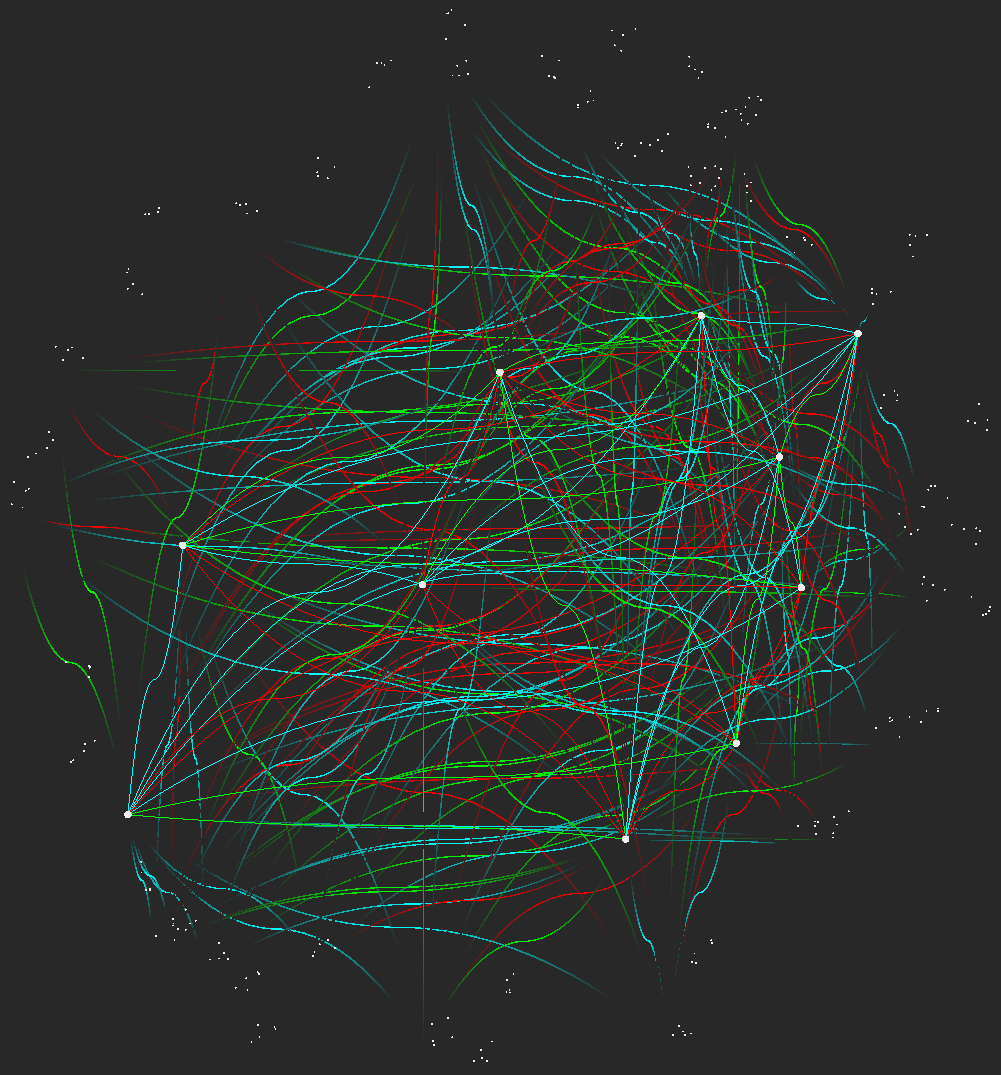
\includegraphics[width=\linewidth]{figRandom.pdf}
	\end{ruledfig}
	
	\begin{proof}
		Suppose we have only $ 2 $ colours (say, red and blue) to use in this problem so, if we pick any vertex we can separate its adjacent edges into these two categories, and as the total number of vertices must be infinite, we must either have one or both categories containing infinite vertices, and so we take whichever is infinite (in case both are, we can take any). If we repeat this process we'll eventually have the set $ A $ we were looking after.
	\end{proof}

	It can be seen as either:
	\begin{enumerate}
		\item a matter of sequences
		
		as this sequence can never converge and so we must have an infinite number of elements in one of the subsets.
		\item as a probability
		
		as the probability of a monochromatic subset happening must be non-zero and it will eventually happen if we iterate the process indefinitely.
	\end{enumerate}
	
	\begin{theorem}[Schur, 1916]\label{thm:schur}
		Let $ c:\mathbb{N}\longrightarrow\set{1,...,r} $ then, there exists $ x,y,z\in\mathbb{N} $ distinct such that they determine a monochromatic sum (aka a \term{Schur triple}), i.e.
		\begin{itemize}
			\item $ x+y=z $
			\item $ c(x)=c(y)=c(z) $.
		\end{itemize}
	\end{theorem}

	\begin{proof}
		Define a $ c':\binom{\mathbb{N}}{2}\longrightarrow \set{1,\ldots,r} $ such that, by \ref{thm:ramsey}, we have an $ A\subset\mathbb{N} $ that's monochromatic. Then, define $ c'(\set{a,b})=c(|a-b|) $, so that we can encode the arithmetic structure of integers, and let $ x<y<z,x,y,z\in A $.
		
		\begin{center}
			
			\begin{tikzpicture}
				\node (a) at (0,0) {$ x $};
				\node (b) at (3,0) {$ y $};
				\node (c) at (6,0) {$ z $};
				
				\draw[-Latex] (a.north) to[out=60,in=120] node[above] {$ c(z-x) $} (c.north);
				\draw[-Latex] (a.north east) to[out=30,in=150] node[above,xshift=4pt] {$ c(y-x) $} (b.north west);
				\draw[-Latex] (b.north east) to[out=30,in=150] node[above,xshift=-4pt] {$ c(z-y) $} (c.north west);
			\end{tikzpicture}
			
		\end{center}
		
		Define
		\begin{align*}
			c(y-x)&=x',\\
			c(z-y)&=y',\\
			c(z-x)&=z'
		\end{align*}
		then $ c(b-a)+c(c-b)=c(c-a) $.
	\end{proof}

	

	Now we define a new quantity, which we shall call
	\begin{definition}[Ramsey number]
		We denote the \term{Ramsey number} of $ k $ vertices by $ R(k)\coloneq\min\set{n:\forall c:E(K_n)\longrightarrow\set{R,B}\exists \textup{ monochromatic copy of }K_k} $.
	\end{definition}

	\note{A complete graph of $ n $ vertices (denoted by $ K_n $) is basically what we get if we draw $ n $ vertices and connect all the possible pairs.}
	
	That is, we define $ R(k) $ as the least number of vertices $ n $ a \term{complete graph} (aka a \term{clique}) must have so that, no matter how we colour it, it will necessarily contain a monochromatic copy of a complete graph of $ k $ vertices.
	
	Which is the exact same problem we introduced before with the party example, as we wished to show that $ R(3)=6 $, that is, only in a complete graph of size $ 6 $ we could guarantee there would be a monochromatic triangle.

	\begin{theorem}[Erdős \& Szekeres, 1935]
		$ R(k)<\infty $ and, actually $ R(k)<2^{2k}=4^{k} $
	\end{theorem}

	\begin{proof}
		In the same way we could guarantee there'd be an infinite monochromatic set in a random colouring of natural pairs (\ref{thm:ramsey}), we can select a vertex $ v_i $ of a clique with $ n $ vertices and divide it into two portions: say red and blue. Then the largest must have at least half ($ -1 $) of the total number of vertices, and if we repeat this process at least $ 2k-1 $ times we can guarantee we'll have a monochromatic $ k $-vertex clique (for the last set must have $ k $ vertices).
		
		%TODO
		\TODO{illustration}
		
		\begin{center}
			\begin{tikzpicture}
				\coordinate (a) at (0,0);
				\coordinate (b) at (1,0);
				\coordinate (c) at (2,0);
				\coordinate (d) at (8,0);
				
				\draw[red] (a) parabola bend ($ (a)!0.5!(d)+(0,1) $)   (d);
				\draw[red] (b) parabola bend ($ (b)!0.5!(d)+(0,0.9) $) (d);
				\draw[red] (c) parabola bend ($ (c)!0.5!(d)+(0,0.8) $) (d);
				
%				\path[name path=Aline] ($ (a)+(0,0.8) $) -- ($ (d)+(0,0.8) $);
%				\path[name path=Bline] ($ (b)+(0,0.8) $) -- ($ (d)+(0,0.8) $);
%				\path[name path=Cline] ($ (c)+(0,0.8) $) -- ($ (d)+(0,0.8) $);
%				
%				\draw[name intersections={of=Aline and A,name intersection=i},papercolor,dashed] (i-1) parabola bend (amid) (i-2);
				
			\end{tikzpicture}
		\end{center}
	\end{proof}

	But we can get a stronger bound by selecting our partitions more carefully.

	\begin{lemma}
		$ R(s,t)\leqslant R(s-1,t)+R(s,t-1) $
	\end{lemma}

	\begin{proof}
		Let $ G $ be a graph with $ n=R(s,t)-1 $ which we will colour with $ c:E(K_n)\longrightarrow\set{R,B} $, such that it doesn't have a {\color{cyan}blue $ K_s $} or a {\color{red}red $ K_t $}. Take $ v\in V(K_n) $ and separate its neighbours into two groups: those which have a blue edge connecting $ v $ to them (say, group $ A $) and the same for those with a red edge (group $ B $). Then we cannot have {\color{cyan} $ K_{s-1} $} or {\color{red} $ K_t $} inside $ A $.
		
		So we must \textit{always} have $ |A|\leqslant R(s-1,t)-1 $ and $ |B|\leqslant R(s,t-1)-1 $ for any step of the recursion (say, take a vertex $ v'\in A $ and apply the same logic for some $ A' $ and $ B' $).
		
		Thus, we have
		\[ |V|=|A|+|B|+1\implies R(s,t)-1=n=|A|+|B|+1\leqslant R(s-1,t)+R(s,t-1)-1. \]
	\end{proof}
	
	Let's now put use the idea of recursion and get a more solid bound
	
	\begin{lemma}
		$ R(s,t)\leqslant \binom{s+t-2}{s-1}\quad\forall s,t\geqslant 2 $
	\end{lemma}

	\begin{proof}
		\TODO{proof by induction \& approx}
	\end{proof}

	Now we might be interested in estimating a lower bound for the Ramsey number, and we can do something pretty quick and dirty which is, basically, to notice that if we take $ k-1 $ red $ (k-1) $-vertex cliques interconnected by blue edges (basically a $ k-1 $ minor) then we'd have a lower bound already, as the biggest clique has $ k-1 $ vertices, whichever its colour may be.
	
	So we have the bounds
	\[ (k-1)^{2}<R(k)=R(k,k)\leqslant \binom{2k-2}{k-1}<\binom{2k}{k}\approx \dfrac{2^{2k}}{\sqrt{k}}, \]
	but we can still get a much better lower bound on this by using non-constructive methods:
	
	\begin{theorem}[Erdős, 1947]
		$ R(k)>\sqrt{2}^{k} $
	\end{theorem}

	\begin{proof}
		We can get a non-constructive proof by randomly colouring a graph, thus, given a colouring $ c,\forall e\in E(K_n) $, we have
		\begin{align*}
			\mathbb{P}(c(e)=R)&=\dfrac{1}{2},\\
			\mathbb{P}(c(e)=B)&=\dfrac{1}{2}.
		\end{align*}
		That is, the probability of colouring the edge in red or blue is the same and is independent from any other edge.
		
		Then, we want to show that $ \mathbb{P}(\nexists \textup{ monochromatic }K_k)>0 $. Given $ X= $\# of monochromatic copies of $ K_k $ in $ K_n $ (i.e. $ X=\set{0,1,2,\ldots} $) then we want to show that the \term{expected value} of $ X $ is zero (i.e. $ \mathbb{E}[X]=0 $). Let the expected value be the weighted sum of all probabilities
		\[ \mathbb{E}[X]=\sum_{k=0}^{\infty}k\,\mathbb{P}(X=k) \]
		then we might derive the linearity property of this operator:
		\[ \mathbb{E}[X+Y]=\mathbb{E}[X]+\mathbb{E}[Y]. \]
		
		Define the \term{indicator function}:
		\[ \mathbb{1}[X]=\begin{cases}
			1,\quad\text{if $ X $ is true}\\
			0,\quad\text{if $ X $ is false}
		\end{cases}. \]
	
		Thus, what we want to evaluate can be written as
		\[ \mathbb{E}[X]=\sum_{K_k\subset K_n}\tikzmark{el}\mathbb{E}\sbr{\mathbb{1}\tikzmark{or}\sbr{K_k \textup{ is monochromatic}}} \]
		
		\begin{tikzpicture}[overlay,remember picture]
			\draw[decorate,decoration={brace,amplitude=4pt,mirror,raise=4pt}] (el) -- node[below=7pt,name=m] {$ =\mathbb{P} $} (or);
			\node[below right=-8pt,text width=7cm, yshift=2pt] at (m.east) {as the expected value of what we want is simply the probability of it happening.};
		\end{tikzpicture}
	
		\medskip
		
		So, we have that the probability of some $ K_k\subset K_n $ being monochromatic is such that each of its edges are the same color, that is $ \binom{k}{2}-1 $ edges ($ -1 $ because the first edge could be whatever and the others have to all be the same). As the probabilities are the same we have $ (1/2)^{\binom{k}{2}-1} $
		\[ \mathbb{E}[X]=\sum_{K_k\subset K_n}\mathbb{P}\sbr{K_k \textup{ is monochromatic}}=\binom{n}{k}\del{\dfrac{1}{2}}^{\binom{k}{2}-1}. \]
		
		Given the inequality \[ \del{\dfrac{n}{k}}^{k}\leqslant\binom{n}{k}\leqslant\del{\dfrac{\mathrm{e}\,n}{k}}^{k} \]
		then, if $ k\ll n $ it follows that $ \binom{n}{k}\approx\del{\mathrm{e}\,n/k}^{k} $ is a good approximation.
		
		Using this inequality we have that
		\[ \mathbb{E}[X]=\del{\dfrac{\mathrm{e}\,n}{k}}^{k}\del{\dfrac{1}{2}}^{\sfrac{k(k-1)}{2}-1}=2\del{\dfrac{\mathrm{e}\,n}{k}2^{-\sfrac{(k-1)}{2}}}^{k}, \]
		and, as we want to show that $ n\leqslant (\sqrt{2})^{k} $, so let $ n=(\sqrt{2})^{k} $, then
		 \[ \mathbb{E}[X]\leqslant 2\del{\dfrac{\mathrm{e}\,2^{k/2}}{k}2^{-\sfrac{(k-1)}{2}}}^{k}=2\del{\dfrac{\mathrm{e}\,\sqrt{2}}{k}}^{k}<1\quad\textup{if }k\geqslant 6, \]
		 which implies that
		 \[ \mathbb{P}\sbr{X=0}>0. \]
	\end{proof}

	\chapter{Extremal graph theory}
	
	\section{A bird's eye view}

	Now, let's define the \term{extremal number} of a graph $ H $ and $ n $ vertices $ \ex(n,H) $ which gives us the maximum number of edges we can have such that a $ n- $vertex graph $ G $ doesn't contain a copy of another graph $ H $. 
	\begin{definition}[extremal number]
		$ \ex(n,H)=\max\set{E(G): H\nsubseteq G\subset K_n} $
	\end{definition}

	Now we might ask the following question:
	\begin{example}
		What is the maximum number of edges a graph can have without any triangles?
	\end{example}
	Which translates to asking ``$ \ex(n,K_3)=? $''.
	
	We can find such a number by first conjecturing on some \textit{edgy} graphs which ought not to have triangles in them, such as these:
	
	% todo
	\TODO{draw some $ K_3- $free graphs}
	
	And we should sometime find that a \term{bipartite graph} (aka, a graph which can be divided into two sets of disconnected vertices with its only edges going between those two groups) might be the optimal answer. That would mean that $ \ex(n,K_3)=\floor{n^{2}/4} $.
	
	% todo
	\TODO{draw a bipartite graph.}
	
	So, let's try and prove this:
	
	\begin{conjecture}
		$ \ex(n,K_3)=\floor{n^{2}/4} $
	\end{conjecture}

	\begin{proof}
		Let $ G $ be the largest $ K_3- $free $ n-$vertex graph.
		
		So, suppose we have $ e(G)\leqslant \floor{n^{2}/4} $, then, if $ K_3\nsubseteq G $ we have
		\begin{itemize}
			\item for $ n=1 $:
			\[ e(G)=0\leqslant \floor{1^{2}/4}=0. \]
			\item for $ n=2 $:
			\[ e(G)=1\leqslant \floor{2^{2}/4}=1. \]
			\item for $ n=3 $:
			\[ e(G)=2\leqslant \floor{3^{2}/4}=2. \]
		\end{itemize}
		
		This hypothesis is equivalent to taking a complete bipartite graph, so we can make a clever construction to get a bound on the number of edges:
		
		We can grab one of its edges $ e\in E(G) $, so that each of $ e $'s vertices determines a disjoint subset, for if they had any vertex in common, there would be a copy of $ K_3 $ contained in $ G $.
		
		Let $ G' $ be this new graph we get by selecting an edge $ e\in E(G) $ and removing it from $ G $.
		
		Let $ G' $ be this new graph we get by selecting an edge $ e\in E(G) $ and removing it from $ G $.
		\TODO{illust of $ G $ and $ G' $}
		
		If $ G $ doesn't contain any copies of $ K_3 $ we can have at most $ n-2 $ vertices between $ e $ and $ G' $ (because there can be no more than one edge between the vertices in $ e $ and $ G' $ without forming a triangle), plus the edge $ e $ we've selected. Thus, by applying an induction on $ n $ we have:
		\begin{align*}
			e(G)&\leqslant e(G')+n-2+1\\
					&\overset{IH}{\leqslant}\floor{\dfrac{(n-2)^{2}}{4}}+n-1=\floor{\dfrac{n^{2}-4n+4+4n-4}{4}}=\floor{\dfrac{n^{2}}{4}}.
		\end{align*}
	\end{proof}

	Now we can study the more general problem, where we want to generalize $ K_3 $ to any $ K_n $. The natural idea is to extend the bipartite graph we saw earlier to a $ r- $partite graph, which we shall call \term{Turán graph} on $ n $ vertices, $ T(n,r) $.

	\begin{theorem}[Turán]
		$ \ex(n,K_{r+1})=\underbrace{e(T(n,r))}_{=t(n,r)}\approx \del{1-1/r}\binom{n}{2} $
	\end{theorem}
	
	\begin{proof}
		So, we can once again use induction to prove this, grabbing instead of an edge, a $ K_{r} $ graph that composes the Turán graph. Then we have the same edge relation as before:
		\begin{align*}
			K_{r+1}\nsubseteq G\implies e(G)&\leqslant e(G')+(n-r)(r-1)+\binom{r}{2}\\
			&\overset{IH}{\leqslant}t(n-r,r)+(n-r)(r-1)+\binom{r}{2}=t(n,r).
		\end{align*}
		
		One can see that $ (n-r)(r-1)+\binom{r}{2} $ is the exact portion that was missing from $ t(n-r,r) $ to prove the induction hypothesis by observing that:...
	
		\TODO{draw graphs showing abstract $ G/G' $ and addition of vertices to $ T(n-r,r) $ and explain better}
	\end{proof}

	Now we might wonder how we could maximize the number of edges without any $ n- $vertex cycle $ C_n $. As $ C_3=K_3 $ we might ask this for $ C_4 $ first:
	
	\[ \ex(n,C_4)=? \]
	
	And quickly we notice there's no reliable construction of a graph which indicates us the solution. Upon noticing this, Erdős came up with a very intuitive and powerful idea: count some object in two different manners.
	
	In this case, he defined a \term{cherry} as a little cute $ 3- $vertex graph which doesn't loop.

	\begin{ruledfig}
		
		\begin{minipage}{0.45\linewidth}
			\center
			\begin{tikzpicture}
				\draw[thin] (0,0) coordinate (a) to[out=200,in=75] (180+60:1) coordinate (b) (a) to[out=320,in=105] (-60:1) coordinate (c);
				\coordinate (ap) at (-0.1,0.3);
				\coordinate (atp) at (0.15,0.3);
				\fill[green] (ap) to[out=100,in=160] +(160:0.6) coordinate (e) (atp) to[out=85,in={180+60}] ($ (atp)+(75:0.6) $) coordinate (d);
				\begin{scope}[rotate=75]
					\fill[green] (atp) parabola bend ($ (0,0)!0.4!(d)+(atp)!0.15!90:(d) $) (d) (atp) parabola bend ($ (0,0)!0.4!(d)+(atp)!0.2!270:(d) $) (d);
				\end{scope}
				\draw[thick,green] (a) to[out=90,in={-10}] ($ (ap)!0.2!(e)+(1pt,0.3pt) $) (a) to[out=90,in={180+75}] ($ (atp)+(60:1pt) $);
				\draw[line width=0.1pt,black] ($ (ap)!0.2!(e)+(0,1pt) $) to[out={90+65},in={-10}] ($ (ap)!0.9!(e)+(0,1pt) $) ($ (atp)!0.15!(d)+(0.4pt,0) $) to[out=85,in={180+70}] ($ (atp)!0.8!(d)+(0.2pt,0) $);
				
				\fill[red] (b) circle (3pt) (c) circle (3pt);
			\end{tikzpicture}
		\end{minipage}\tikzmark{ar1}
		\hfill
		\begin{minipage}{0.45\linewidth}
			\center
			\begin{tikzpicture}
				\draw[thin] (0,0) coordinate (a) -- (180+60:1) coordinate (b) (a) -- (-60:1) coordinate (c);
				
				\fill[red] (b) circle (3pt) (c) circle (3pt);
				\fill[green] (a) circle (2pt);
			\end{tikzpicture}
		\end{minipage}
		
		\begin{tikzpicture}[overlay, remember picture]
			\draw[-{Implies[length=5pt,width=8pt]},double distance=5pt] ($(ar1)+(-0.3,0)$) -- +(1,0);
			\fill[papercolor] ($(ar1)+(-0.3,-2.3pt)$) rectangle +(0.8,4.6pt);
		\end{tikzpicture}
		
		\vspace{0.1cm}
	\end{ruledfig}

	And then we can see a $ C_4 $ as two cherries glued together:

	\begin{ruledfig}
		
		\begin{minipage}{0.45\linewidth}
			\center
			\begin{tikzpicture}
				\draw[thin] (0,0) coordinate (a) -- ++(1,0) coordinate (b) -- ++(0,1) coordinate (c) -- ++(-1,0) coordinate (d) -- cycle;
				
				\fill[red] (a) circle (3pt) (c) circle (3pt);
				
				\fill[green] (b) circle (2pt) (d) circle (2pt);
			\end{tikzpicture}
		\end{minipage}\tikzmark{ar2}
		\hfill
		\begin{minipage}{0.45\linewidth}
			\center
			\begin{tikzpicture}
				\draw[thin] (0,0) coordinate (a) ++(1,0) coordinate (b) ++(0,1) coordinate (c) ++(-1,0) coordinate (d);
				\draw[thin] (d) -- (a) (d) -- (b) (c) -- (a) (c) -- (b);
				
				\fill[red] (a) circle (3pt) (b) circle (3pt);
				
				\fill[green] (c) circle (2pt) (d) circle (2pt);
			\end{tikzpicture}
		\end{minipage}
		
		\begin{tikzpicture}[overlay, remember picture]
			\draw[-{Implies[length=5pt,width=8pt]},double distance=5pt] ($(ar2)+(-0.3,0)$) -- +(1,0);
			\fill[papercolor] ($(ar2)+(-0.3,-2.3pt)$) rectangle +(0.8,4.6pt);
		\end{tikzpicture}
		
		\vspace{0.1cm}
	\end{ruledfig}
	
	Thus we have that the number of cherries on a graph (if we count its vertices from above) is the sum of the pairs which can be formed by any $ v\in V(G) $. The idea of neighbours can be elegantly expressed as the \term{degree} $ d(v) $ of a vertex, so that we have
	\[ \textup{\# cherries }=\sum_{v\in V(G)}\binom{d(v)}{2}. \]
	Then, if we count from below, we have an upper bound for the number of cherries, as each pair can form only one cherry at most, as if they formed more than one cherry we'd have a $ C_4 $.
	
	Thus, we have
	\begin{align*}
		n^{2}\geqslant\binom{n}{2}\geqslant\textup{\# cherries}&=\sum_{v\in V(G)}\binom{d(v)}{2}\\
		\intertext{and by Jensen's inequality\footnotemark.}
		\textup{\# cherries}&\geqslant n\binom{\sum d(v)/n}{2}\\
		\intertext{and then, as we count every edge twice when summing all of their degrees, we have}
		&=n\binom{2e(G)/n}{2}=\dfrac{n}{2}\del{\dfrac{2e(G)}{n}}\del{\dfrac{2e(G)}{n}-1}\\
		n^{2}\geqslant\textup{\# cherries}&\geqslant \dfrac{1}{n}e(G)^{2}\\
		\implies e(G)&\leqslant n^{3/2}.
	\end{align*}

	And then we have that $ \ex(n,C_4)\leqslant n^{3/2} $.
	
	\footnotetext{This inequality talks about convexity. See it at \url{https://brilliant.org/wiki/jensens-inequality}.}
	
	Then we might ask ``for which graphs $ H $ do we have $ \ex(n,H)=\theta(n^{2}) $ (i.e. $ \ex(n,H)\geqslant c\,n^{2} $)?''
	
	We can see that, if $ H $ isn't contained by a larger bipartite graph (thus $ H $ itself cannot be bipartite) then it has $ \ex(n,H)\geqslant n^{2}/4 $.
	
	\begin{theorem}[Erdős 1935, Kővári--Sós--Turán 1950's]
		$ \ex(n,H)=o(n^{2}) $
	\end{theorem}

	\TODO{explain $ o $ notation. write Erdos proof more concisely above}
	
	\begin{proof}
		We can start by noticing that, given a bipartite graph $ H $ it must fit into another, larger, bipartite graph with disjoint sets of sizes $ s $ and $ t $, denoted $ K_{s,t} $. So we can write the inequality
		\[ \ex(n,H)\leqslant \ex(n,K_{s,t}) \]
		so now we can focus on bounding $ \ex(n,K_{s,t}) $ from below, which can be done by generalizing the idea from the previous proof (for $ C_4 $), only this time we'll be counting $ s- $cherries:
		
		\begin{ruledfig}
			
			\center
			\begin{tikzpicture}
				\coordinate (a) at (0,0);
				\coordinate (b) at (-1.5,-1);
				\coordinate (c) at (-0.4,-1);
				\coordinate (d) at (0.8,-1);
				\coordinate (e) at (2,-1);
				
				\draw[thin] (a) -- (b) (a) -- (c) (a) -- (e);
				\draw[thin,dashed] (a) -- (d) (a) -- ($ (d)+(0.5,0) $) (a) -- ($ (d)+(-0.5,0) $);
				\foreach \i in {1,...,10}{
					\draw[thin,dashed] (a) -- ($ (d)+(0.5*rand,0) $);
				}
				
				\fill[red] (b) circle (2pt) (c) circle (2pt) (e) circle (2pt);
				\foreach \i in {1,...,30}{
					\fill[red] ($ (d)+(0.6*rand,0) $) circle (0.8pt);
				}
				\fill[green] (a) circle (2pt);
				
				\draw[decorate,decoration={brace,amplitude=10pt,mirror,raise=5pt}] ($ (b)+(-2pt,0) $) -- node[below=15pt] {$ s $} ($ (e)+(2pt,0) $);
			\end{tikzpicture}
			
		\end{ruledfig}
	
		
		\begin{align*}
			\del{\dfrac{n}{s}}^{s}\geqslant (t-1)\binom{n}{s}\geqslant\textup{\# cherries}&=\sum_{v\in V(G)}\binom{d(v)}{s}\\
			\intertext{again, by Jensen's inequality}
			\textup{\# cherries}&\geqslant n\binom{\sum d(v)/n}{s}=n\binom{2e(G)/n}{s}\\
			&= \dfrac{n}{s!}\del{\dfrac{2e(G)}{n}}\del{\dfrac{2e(G)}{n}-1}\cdots \del{\dfrac{2e(G)}{n}-s+1}\\
			\del{\dfrac{n}{s}}^{s}\geqslant\textup{\# cherries}&\geqslant \dfrac{e(G)^{s}}{s^{s}\,n^{s-1}}\\
			\implies e(G)&\lesssim C\,n^{2-1/s}.
		\end{align*}
	
		So that $ \ex(n,H)\lesssim C\,n^{2-1/s} $.
	\end{proof}

	
	\chapter{Trees \& Planar Graphs}
	
	\begin{definition}
		A tree is a connected graph without cycles \\ \textit{or}
		
		maximal graph without cycles \\ \textit{or}
		
		minimal connected graph
	\end{definition}

	\begin{lemma}\label{lem:l1trees}
		Let $ G $ be a graph with average degree $ d $ then $ \exists G'\in G $ with a minimum degree ($ \delta $) $ x=x(d)\geqslant d/2 $
	\end{lemma}
	
	\begin{proof}
		\begin{center}
			\begin{tikzpicture}
				\path[draw,use Hobby shortcut,closed=true,shift={(-7,-0.2)}]
				(-.4,0) .. (-.6,.3) .. (-.5,.6) .. (-.3,-.3);
				\fill[cyan] (-6.8,0) node[left=0pt] {$ T' $} coordinate (p) circle (1pt);
				\draw[cyan] (p) node[below] {$ u $} -- +(0.5,0.2) circle (1pt) node[right] {$ v $};
				\draw[decorate,decoration={brace,amplitude=5pt,mirror}] (-7.5,-0.8) -- node[below=10pt] {$ T $} +(1.5,0);
				
				\draw[-{Implies[length=5pt,width=8pt]},double distance=5pt] (-5.5,0) -- +(1,0);
				\fill[papercolor] ($(-5.5,0)+(-0.3,-2.3pt)$) rectangle +(1.1,4.6pt);
				
				\path[draw,use Hobby shortcut,closed=true,rotate=90]
				(0,0) .. (.5,1) .. (1,3) .. (.3,4) .. (-1,2) .. (-1,.5);
				\draw (-1.5,.3) node[] {$ G' $};
				\path[draw,use Hobby shortcut,closed=true,shift={(-3,-0.2)}]
				(-.4,0) .. (-.6,.3) .. (-.5,.6) .. (-.3,-.3);
				\fill[cyan] (-2.8,0) node[left=0pt] {$ T' $} coordinate (pp) circle (1pt);
				\draw[cyan] (pp) node[below] {$ u $} -- +(0.5,0.2) circle (1pt) node[right] {$ v $};
				\draw[->] (pp)+(0,-0.5) to[out={180+30},in={180-30}] +(0.2,-1.5) node[below right] {\footnotesize $ D(T')\leqslant k-2 $ but $ \delta(G')\geqslant k-1 $};
			\end{tikzpicture}
		\end{center}
	
		If every vertex has less than $ x $ edges going forwards ($ \rightarrow $) than we must have at most $ n\,d/2=e(G)\leqslant x\,n\implies x>d/2 $.
	\end{proof}

	\begin{lemma}\label{lem:l2trees}
		Let $ G $ be a graph with minimum degree $ \delta(G)\geqslant k-1 $. Then $ T\subset G\forall $ trees $ T $ with $ k $ vertices.
	\end{lemma}

	\begin{proof}
		Induction in $ k $. For $ k=1,2 $. Take a maximal path inside a tree.
		
		\TODO{organize the proof and draw an abstract maximal path}
		
		If $ T $ has $ k $ vertices, take out a leaf:
		
		\TODO{illustration of proof}
		
		So, it follows that $ d(u)\geqslant\delta(G)=k-1 $.
	\end{proof}
	
	\[ e(G)=C\,n=\bar{d}(G)=2C\overset{\overset{(\ref{lem:l1trees})}{\exists G'\subset G}}{\implies}\delta(G')\geqslant C\overset{\overset{(\ref{lem:l2trees})}{\exists T\subset G'}}{\implies} \]
	
	Let $ T $ be a tree with a fixed number of vertices $ k $. If we wish to bound $ \ex(n,T) $ we then have
	\[ (k-2)\dfrac{n}{2}\leqslant \ex(n,T)\leqslant (k-1)n \]
	
	\begin{theorem}
		$ \ex(n,H)=O(n)\iff H $ doesn't have cycles
	\end{theorem}

	\begin{proof}
		$ (\leftarrow) H $ doesn't have cycles $ \implies H\subset T $ tree
		
		\[ \ex(n,H)\leqslant\ex(n,T)=O(n) \] 
	\end{proof}

	So we actually want to prove that
	
	\begin{theorem}
		$ \ex(n,C_{2k})\gg n $
	\end{theorem}

	\begin{definition}[The random Erdős–Rényi graph]
		$ G(n,p) $ has $ n $ vertices and, every possible edge on this graph has probability $ p $ of actually existing. 
	\end{definition}

	Notice that this is actually a probability distribution on graphs with $ n $ vertices, but we can use it as a function.
	
	Let $ p=p(n),n\to\infty $, and then we choose some $ p(n) $ that satisfies:
	\begin{itemize}
		\item $ e(G(n,p))\gg n $
		\item $ C_{2k}\nsubseteq G(n,p) $
	\end{itemize}

	We could construct this by analysing the expected value function
	\[ \mathbb{E}\sbr{e\del{G(n,p)}}=\sum_{e\in E(K_n)}\overbrace{\mathbb{P}\del{e\in G(n,p)}}^{p}=\binom{n}{2}p. \]
	
	\begin{align}
		e(G(n,p))&\sim\mathrm{Bin}\del{\binom{n}{2},p}\nonumber\\
		&\approx p\,n^{2}\quad\text{very likely}\nonumber\\
		&\implies p\gg \dfrac{1}{n}\nonumber\\
		&\implies p\,n\to\infty\label{eq:tiexp}
	\end{align}

	\[ X=\textup{\# of copies of }C_{2k}\in G(n,p) \]
	\[ \mathbb{E}\sbr{X}=\sum_{C_{2k}\in K_n} \mathbb{P}\del{C_{2k}\in G(n,p)}\approx p^{2k}n^{2k}=(p\,n)^{2k}\overset{\textup{by \ref{eq:tiexp}}}{\longrightarrow}\infty \]
	
	Fail! But, as it increases slowly. Choose $ p=p(n) $ such that $ (p\,n)^{2k}\ll p\,n^{2}\iff p^{2k-1}\,n^{2k-2}\ll 1\implies p\ll n^{-1+1/(2k-1)} $.
	
	\begin{lemma}
		Let $ p=n^{-1+\varepsilon} $, we want $ p $ such that:
		\begin{itemize}
			\item\label{item:ineq1} $ e\del{G(n,p)}\geqslant p\,n^{2}/100 $
			\item\label{item:ineq2} $ \# C_{2k}\in G(n,p)\overset{?}{\leqslant}(p\,n)^{2k} $
		\end{itemize}
	\end{lemma}

	To justify such inequalities we have
	\begin{enumerate}
		\item Chernoff inequality
		\[ \mathbb{P}\del{\envert{\mathrm{Bin}(N,p)-p\,N}>t}\leqslant \mathrm{e}^{-t^{2}/(2p\,N)} \]
		
		\item Markov's inequality
		Given a random variable $ X\in\set{0,1,...} $ we have
		\[ \mathbb{P}\del{X\geqslant t}\leqslant \mathbb{E}\sbr{X}/t \]
		
		\begin{proof}
			\begin{align*}
				\mathbb{E}[X]&=\sum_{k=0}^{\infty}k\,\mathbb{P}\del{X=k}\geqslant \sum_{k=t}^{\infty}k\,\mathbb{P}\del{X=k}\\
				&\geqslant \sum_{k=t}^{\infty}t\,\mathbb{P}\del{X=k}=t\,\mathbb{P}\del{X\geqslant t}\\
				\implies \mathbb{P}\del{X\geqslant t}&= \mathbb{E}[X]/n
			\end{align*}	
		\end{proof}
	\end{enumerate}
	
	\begin{definition}[Planar graph]
		A graph is planar if it can be drawn without crossing edges
	\end{definition}

	If $ G $ is planar what is the upper bound on $ e(G) $.
	
	\begin{lemma}
		$ V+F=E+2 $
	\end{lemma}

	Let $ G $ be a planar connected graph $ v(G)\geqslant 1 $.
	
	So $ v(G)+f(G)=e(G)+2 $, and by induction on $ e(G) $ we have.
	\[ e(G)=0,v(G)=1,f(G)=1\checkmark \]
	
	Case 1. If there's a vertex $ v $ with degree $ 1 $, then remove $ v $.
	\begin{gather*}
		v(G)\to v(G)-1\\
		e(G)\to e(G)-1\\
		f(G)\to f(G)
	\end{gather*}

	Case 2. If there's no leaf in $ G $, there's a cycle in $ G $, thus remove an edge $ j $ from the cycle.
	\begin{gather*}
		v(G)\to v(G)\\
		e(G)\to e(G)-1\\
		f(G)\to f(G)-1
	\end{gather*}

	$ G' $ is connected: if a path didn't use $ j $, then nothing's changed else it use the rest of the cycle.
	
	Let $ G $ be planar \& maximal $ \implies $ connected.
	\[ \implies n+f(G)=e(G)+2\,,\,3f(G)\leqslant 2e(G)\,,\,e(G)\leqslant 3n-6 \]
	
	\begin{corollary}
		$ K_5 $ isn't planar
	\end{corollary}

	\begin{proof}
		\[ v(K_5)=\binom{5}{2}>15-6=9 \]
	\end{proof}

	\begin{corollary}
		$ K_{3,3} $ isn't planar
	\end{corollary}
	
	\begin{proof}
		If the graph is triangle free (as it is bipartite), we have that $ 2e(G)\geqslant 4f(G)\implies e(G)\leqslant 2n-4 $.
		
		\[ v(K_{3,3})=\binom{6}{2}-2\binom{3}{2}=9>12-4=8 \]
	\end{proof}

	\begin{definition}[Chromatic number]
		\[ \chi(G)=\min\set{r:\exists c:v(G)\longrightarrow\set{1,...,r}\textup{ such that }c(u)\neq c(v)\forall u,v\in E(G)} \]
	\end{definition}

	\begin{theorem}
		$ G $ is planar $ \iff \nexists $ a topological copy of $ K_5 $ or $ K_{3,3} $
		and $ \iff \nexists K_5 $ or a $ K_{3,3}- $minor in $ G $.
	\end{theorem}

	\TODO{illust topological copy and minors}
	
	\begin{definition}
		$ \Gamma(G,H)=\min\set{n:\forall e(K_n)\longrightarrow \set{R,B}\exists {\color{red} G} \textup{ or }{\color{cyan} H}} $
	\end{definition}

	\begin{theorem}[4-colour theorem]
		If $ G $ is planar, then $ \chi(G)\leqslant 4 $
	\end{theorem}
		
	\begin{theorem}
		If $ G $ is planar, then $ \chi(G)\leqslant 6 $
	\end{theorem}

	\begin{proof}
		By induction on $ n=|v(G)|,e(G)\leqslant 3n-6\implies \delta(G)\leqslant 5 $
	\end{proof}

%	\part{Misc}

	\begin{theorem}
		If $ p\geqslant (1+\varepsilon)\log n/n $ then $ G(n,p) $ is connected with high probability.
	\end{theorem}
	
	\begin{proof}
		If we define a random variable as the number of non-edges between some connected part of our graph and the rest of the graph (number of edges of a $ K_{k,n-k} $ bipartite graph in $ \overline{G(n,p)}=G(n,(1-p)) $), i.e.
		\[ X_k=\# K_{k,n-k}\subset \overline{G(n,p)} \]
		so that if the expected value of $ X_k $ goes to zero $ \forall k\in[n/2] $ with $ n $ increasing we have exactly what we want:
		\begin{align*}
			\mathbb{E}[X_k]&=\underbrace{\binom{n}{k}}_{\text{select $ k $ vertices for some $ k- $set}}(1-p)^{k(n-k)}\\
			\intertext{approximating $ (1-p)^{k(n-k)} $ by $ \exp(-p\,k(n-k)) $ and $ \binom{n}{k} $ as $ \del{\mathrm{e}n/k}^{k} $ we have}
			&=\del{\dfrac{\mathrm{e}n}{k}}^{k}\exp\del{-p\,k(n-k)}=\del{\dfrac{\mathrm{e}n}{k}\mathrm{e}^{-p(n-k)}}^{k}\\
			\intertext{taking $ p\geqslant (1+\varepsilon)\log n/n $ we have}
			\mathbb{E}[X_k]&\leqslant\del{\dfrac{\mathrm{e}n}{k}\exp\del{-(1+\varepsilon)\log n(n-k)/n}}^{k}\\
			\intertext{as $ \mathrm{e}^{\log n}=n $ we have}
			&\leqslant\del{\dfrac{\mathrm{e}n}{k}n^{-(1+\varepsilon)(n-k)/n}}^{k}
		\end{align*}
		we want this to be small, so we must analyse $ 2 $ cases:
		\begin{enumerate}
			\item $ k=o(n) $:
			In this case, the exponential with $ (n-k)/n\approx 1 $, thus $ n^{1-(1+\varepsilon)}=n^{-\varepsilon} $ which is already small.
			\item $ k=\Theta(n) $:
			In this case the exponential is at most $ n^{-(1+\varepsilon)/2} $ (for $ k=n/2 $), and the fraction in $ (\mathrm{e}n/k)\cdot n^{-(1+\varepsilon)/2} $ is basically a constant, so we only need that the exponential term gets smaller than a constant. Then $ n $ is at most $ n^{1-(1+\varepsilon)/2}=n^{1/2-\varepsilon/2} $.
		\end{enumerate}
		Thus, taking only non-constant terms we have
		\[ \mathbb{E}[X_k]\leqslant n^{-k\,\varepsilon/2}. \]
		
		Now we can analyse the probability $ G(n,p) $ isn't connected by the union bound:
		\begin{align*}
			\mathbb{P}\del{G(n,p)\textup{ isn't connected}}&\leqslant\sum_{k=1}^{n/2}\mathbb{P}\del{X_k\geqslant1}\\
			&\leqslant\sum_{k=1}^{n/2}n^{-k\,\varepsilon/2}\\
			\intertext{as this is a summation of a geometric series with ratio $ <1 $, let $ \alpha=n^{-\varepsilon/2} $ and set an upper bound as the summation from $ k=1 $ to $ \infty $:}
			&\leqslant\sum_{k=1}^{\infty}\alpha^{k}=\alpha\del{\dfrac{1}{1-\alpha}}\leqslant 2\alpha
		\end{align*}
		as $ 1-\alpha\leqslant 1/2 $ for $ (1/n)^{\varepsilon/2}\overset{!}{\geqslant} 1/2 $ for any $ \varepsilon/2<1 $ and $ n>1 $.
		
		Thus
		\[ \mathbb{P}\del{G(n,p)\textup{ isn't connected}}\leqslant 2n^{-\varepsilon/2}\overset{\textup{as }n\to\infty}{\to} 0. \]
	\end{proof}

	\begin{theorem}[Erdős \& Stone]
		$ \ex(n,H)=\del{1-\dfrac{1}{\chi(H)-1}+o(1)}\binom{n}{2} $
	\end{theorem}
	\begin{lemma}
		Let $ m\in\mathbb{N},\varepsilon>0 $ such that $ \varepsilon\binom{n}{2}\geqslant\binom{m_0}{2} $ and $ G $ be a graph with density $ e(G)/\binom{n}{2}\geqslant \beta $ thus $ \exists G^{\star}\subset G $ with $ m $ vertices and $ \delta(G^{\star})\geqslant(\beta-\varepsilon)m $.
	\end{lemma}
	\begin{proof}
		...
	\end{proof}
	\begin{lemma}
		...
	\end{lemma}
	\begin{proof}
		...
	\end{proof}
	Now let's prove the theorem
	\begin{proof}
		...
	\end{proof}
	
	
	\chapter{Hypergraphs}
	
	The \term{Ramsey number for hypergraphs} can be defined as
	\begin{definition}[Ramsey number (for hypergraphs)]
		\[ R^{(k)}_r(m)=\min\set{n\colon\forall c\colon\binom{[n]}{k}\longrightarrow[r]\exists \textup{ copy of a monochromatic }K^{(k)}_m} \]
	\end{definition}
	Going through this statement one definition at a time we have that
	\[ \binom{[n]}{k}=\set[2]{S\subset\underbrace{\set{1,\ldots,n}}_{=[n]}\colon |S|=k} \]
	and $ K^{(k)}_m $ denotes a complete $ k- $uniform hypergraph with $ m $ vertices so that we have
	\[ v(K^{(k)}_m)=m \]
	and
	\[ e(K^{(k)}_m)=\binom{m}{k}. \]
	
	\begin{theorem}[Ramsey, 1930]
		$ R^{(k)}_r(m)<\infty\forall k,r,m\in\mathbb{N} $
	\end{theorem}
	\begin{proof}
		\begin{itemize}
			\item $ k=1: $ pigeonhole principle.
			\item $ k=2: $ classic proof.
			\item $ k=3: $...
		\end{itemize}
	
		HI:...
	\end{proof}

	\begin{theorem}[Erdős \& Hajnal]
		$ 2\leqslant R^{(3)}(m)\leqslant 2^{\binom{R(m)}{2}} $
	\end{theorem}
	\begin{proof}
		
	\end{proof}
	
	\section{Happy ending problem}
	
	\begin{definition}
		\[ f(k)=\min\set{n\colon\forall n\textup{ points in }\mathbb{R}^{2} \textup{ generally }\exists k \textup{ points in convex position}} \]
	\end{definition}
	
	\begin{theorem}[Erdős \& Szekeres, 1935]
		$ f(k)\leqslant R^{(4)}(k)\leqslant 2^{2^{2^{C\,m}}} $
	\end{theorem}
	\begin{proof}
		...
	\end{proof}
	
	Let a $ k- $AP be an arithmetic progression of size $ k $. Denote that by
	\[ AP_k(a,d)=\set{a,a+d,\ldots,a+(k-1)d}. \]
	
	\begin{definition}[Van der Waerden number]
		\[ W(r,k)=\min\set{n\colon \forall c\colon [n]\longrightarrow [r]\exists \textup{ a monochromatic} k-\textup{AP}} \]
	\end{definition}
	
	\begin{theorem}[Van der Waerden, 1927]
		$ W(r,k)<\infty $
	\end{theorem}
	\begin{proof}
		For a $ 2- $AP we have Schur's theorem \ref{thm:schur}...
	\end{proof}

	\chapter{Random Graphs}
	
	For $ \mathbb{P}\del{H\subset G(n,p)}\approx ? $
	
	Define $ V(G(n,p))=[n] $ and let $ \mathbb{P}\del{e\in E\del{G(n,p)}}=p,\forall e\in E(K_n) $ independently.
	
	For example, for $ H=K_3 $ let $ X=\# $ of copies of $ K_3 $ in $ G(n,p) $, so
	\[ \mathbb{E}\sbr{X}=\sum_{K_3\subset K_n} p^{3}=\binom{n}{3}p^{3} \]
	
	\[ \mathbb{P}(X\geqslant 1)\overset{\textup{by Markov}}{\leqslant} \mathbb{E}[X]\leqslant p^{3}\,n^{3}\to 0\quad\text{if }p\,n\to 0 \]
	
	\begin{proposition}
		If $ p\ll 1/n $ then $ \mathbb{P}\del{K_3\subset G(n,p)}\to 0 $
		
		$ \iff K_3\nsubseteq G(n,p) $ with high probability.
		
		If $ p\gg 1/n $ (i.e. $ p\,n\to\infty $) then $ \mathbb{E}[X]=\binom{n}{3}p^{3}\to\infty $
	\end{proposition}

	Inequalities. $ X\in\set{0,1,2,\ldots} $
	
	Markov. \[ \mathbb{P}(X\geqslant a)\leqslant \dfrac{\mathbb{E}[X]}{a} \]
	
	Chebyschev \[ \mathbb{P}\del{\abs{X-\mathbb{E}[X]}\geqslant t}\leqslant \dfrac{\Var(X)}{t^{2}} \]
	
	By Markov (taking $ a=t^{2} $ and $ X=\Var(X)=(X-\mathbb{E}[X])^{2} $).
	
	\begin{align*}
		\Var(X)&=\mathbb{E}\sbr{\del{X-\mathbb{E}[X]}^{2}}=\mathbb{E}\sbr{X^{2}-2X\,\mathbb{E}[X]+\mathbb{E}[X]^{2}}\\
		&=\mathbb{E}\sbr{X^{2}}+\mathbb{E}\sbr[2]{-2X\,\underbrace{\mathbb{E}[X]}_{\textup{const}}}+\mathbb{E}\sbr{\mathbb{E}[X]^{2}}=\mathbb{E}\sbr{X^{2}}-2\mathbb{E}[X]^{2}+\mathbb{E}[X]^{2}\\
		\Var(X)&=\mathbb{E}\sbr{X^{2}}-\mathbb{E}\sbr{X}^{2}
	\end{align*}

	\begin{proposition}
		If $ p\gg 1/n $, then $ \mathbb{P}\del{K_3\subset G(n,p)}\to1 $.
	\end{proposition}
	\begin{proof}
		...
	\end{proof}
	
	\begin{proposition}
		If $ p\ll n^{-2/(r-1)} $ then $ \mathbb{P}\del{K_r\subset G(n,p)}\to0 $
	\end{proposition}
	\begin{proof}
		...
	\end{proof}

	\begin{proposition}
		If $ p\gg n^{-2/(r-1)} $ then $ \mathbb{P}\del{K_r\subset G(n,p)}\to1 $
	\end{proposition}

	Sprinkling...
	
	
	
\end{document}